
\documentclass[11pt]{article}
\usepackage{geometry}                % See geometry.pdf to learn the layout options. There are lots.
\geometry{letterpaper}                   % ... or a4paper or a5paper or ... 
%\geometry{landscape}                % Activate for for rotated page geometry
%\usepackage[parfill]{parskip}    % Activate to begin paragraphs with an empty line rather than an indent
\usepackage{doublespace}
\usepackage{graphicx}
\usepackage{amssymb}
\usepackage{epstopdf}
\usepackage{listings}

\usepackage{algorithm,algorithmic}
\DeclareGraphicsRule{.tif}{png}{.png}{`convert #1 `dirname #1`/`basename #1 .tif`.png}

\newtheorem{thm}{Theorem}[section]
\newtheorem{adef}[thm]{Definition}
\newtheorem{cor}[thm]{Corollary}
\newtheorem{lem}[thm]{Lemma}


\title{Quartz Renaissance Solutions on Independent Component Analysis}
\author{Dan Beatty}

\section{Introduction}

\section{Independent Component Analysis Family of Estimators}\label{mutual-independence}
The Independent Component Analysis (ICA) family of estimators are unique regarding the items to be estimated.   The standard ICA form, originally derived in \cite[151]{appo-ica-book} , is shown in equation \ref{standardICA}.  The dataset denoted by $\vec{x}$ is the only observed part.  The mixing matrix ($\mathbf{A}$), the ICs ($\vec{s}$), and the noise ($\vec{\nu}$) are all estimated.  If $\vec{\nu}$ can be assumed to be normal, then it can be eliminated from the standard ICA form to give the %standard 
noiseless ICA form, equation \ref{standardICANoiseless}.  The inverse of the noiseless form allows for estimators of ICA to be constructed.  
%\label{mutual-independence}
%Standard form of ICA w/o noise
\begin{eqnarray}
\vec{x} = \mathbf{A}\vec{s} + \vec{\nu} \label{standardICA} \\
\vec{x} = \mathbf{A}\vec{s} \label{standardICANoiseless} \\
\vec{s} = \mathbf{A}^{-1} \vec{x} \label{standardICAInverse} 
\end{eqnarray}

%Establish linear combinations that become the mixing matrix.  
Construction of an ICA estimator from equation \ref{standardICAInverse} requires a few algebraic manipulations, which are shown in equations \ref{unwhitenedICA} through \ref{whitenedICs}.
$\mathbf{A}\vec{b}$ maximizes $y$'s non-normal characteristics.  Such a $\vec{b}$ makes $\vec{q}$ have only one non-zero component. Therefore, $y$ is an independent component.  Determining the non-normal characteristics is complicated by %has to contend with 
$\pm s_i$ which are the IC(s) determined up to a sign. 
The determination of $\vec{b}$ becomes an angle between vectors.
\begin{eqnarray}
y = \vec{b}^T \vec{x} \label{unwhitenedICA} \\
y = \vec{b}^T \mathbf{A}\vec{s} \\
\vec{q} = \mathbf{A}^{T} \vec{b} \\
y = \vec{q}^T \vec{s} \label{whitenedICs}
\end{eqnarray}

One method for determining the non-normal characteristics is by kurtosis, shown in equation \ref{kurtosisStandardWhite}.  If $y$ is a whitened source of data, then equation \ref{kurtosisStandardWhiteAssumed} holds.
%Non-Normal Character by Kurtosis
\begin{eqnarray}
\kappa _4 (y) = E \{ y^4 \} - 3 (E\{ y^2\})^2 \label{kurtosisStandardWhite}\\
E\{ y^2\} =1 \Rightarrow \kappa _4 (y) = E \{ y^4 \} - 3 \label{kurtosisStandardWhiteAssumed}%\\
%\kappa_4(y)  = m_4 (y)
\end{eqnarray}
The measure of non-normal characteristics can be accomplished by $|\kappa_4(\dot)|$ or $\kappa_4 (\dot) ^2$.  %Note these properties:
Kurtosis has both additive and scaling properties, as shown in equations \ref{addKurtosis} and \ref{scaleKurtosis}:
\begin{eqnarray}
\kappa_4(x_1) + \kappa_4(x_2) \equiv k_4(x_1 + x_2) \label{addKurtosis}\\
\kappa_4(\alpha x) = \alpha \kappa_4 (x) \label{scaleKurtosis}
\end{eqnarray}

The objective is to apply kurtosis to $y$ (or to its definition as an IC element).  Equation \ref{kurtosisAppliedToICACharacter} shows the application of kurtosis to the characteristic, whitened equation of ICA.  A consequence of the data being whitened, shown in equation \ref{consequenceOfICACharacter}, is a reduction of terms for the characteristic equation,   %From this consequence, 
by which the objective of finding each mixing vector translates to determining the unit circle of  the maxima of $\kappa_4 (y)$.  In order to find the unit circle maxima, an assumption shown in equation \ref{icAssumptionUnitCircle}, the kurtosis of each IC is restricted to unit length.  
Therefore, gradient methods can be used to determine the kurtosis.
\begin{eqnarray}
\kappa_4(y) = \sum _i q_i \kappa_4 (s_i) \label{kurtosisAppliedToICACharacter}\\ 
E\{y^2 \} =1 \Rightarrow \sum_i q_i ^2 =1 \label{consequenceOfICACharacter} \\
\kappa_4(s_i) = 1 \Rightarrow F(\vec{q}) = \sum_i q_i ^4 \label{icAssumptionUnitCircle}
\end{eqnarray}


\subsection{Kurtosis Gradient Maximization}
Let $\vec{z}$ be $\vec{x}$ whitened and $\vec{w}$ be a whitened version of $\vec{b}$. Equations \ref{kurtosis-vec-prod} through \ref{kurtosis-vec-prod-to-zero} show how to derive the extreme points via kurtosis.  
If the partial derivative in equation  \ref{kurtosis-vec-prod-to-zero} is set to zero, then the determining the optimal $\vec{w}$ is reduced to determining the roots of $\kappa_4(y)$, which are the maxima and minima.  Note that $\vec{w}$ must be normalized in  each iteration.  Also, the expectation operator, $E(\cdot)$, in many cases, is treated as the classic mean of the argument inside.  %If the partial derivative in equation  \ref{kurtosis-vec-prod-to-zero} is set to zero, then the determining the optimal $\vec{w}$ is reduced to determining the roots of $\kappa_4(y)$, which are the maxima and minima.   Note cite Hyvarian's version of this.
An algorithmic representation of Kurtosis Gradient Maximization is realized in Projection Pursuit show in Algorithm \ref{alg:Projection-Pursuit}.
\begin{eqnarray}
y = \vec{w}^T \vec{z} \\ 
\kappa_4 (y) = \sum _i w_i \kappa_4{z_i} \label{kurtosis-vec-prod} \\
\frac{\partial \kappa _4 (y)} {\partial \vec{w}} = 4 \textrm{sign} (\kappa _4 (y))E\{ \vec{z} (\vec{w}^T \vec{z})^3\} - 3 \frac{\vec{w}}{||\vec{w}||}  \\
\frac{\partial \kappa _4 (y)} {\partial \vec{w}} \approx 4 \textrm{sign} (\kappa_4(y))E \{ \vec{z} (\vec{w}^T \vec{z}) \} \\
\frac{\partial \kappa _4 (y)} {\partial \vec{w}} \to 0 \label{kurtosis-vec-prod-to-zero}
\end{eqnarray}

%  Note that $\vec{w}$ must be normalized each iteration.  Also, the expectation operator in many cases is treated as the classic mean of the argument inside.  

%Note that if M = 1 and N > 1, then Projection Pursuit can only calculate X^T, not X itself. 
% Therefore $y = E (\vec{w}^T \vec{z}) = \vec{w}^T \vec{z}$, and $\Delta \vec{w} = E \{ y^3 \vec{z} \} = y^3 \vec{z}$.

% Supply algorithm here.

\begin{algorithm}
\caption{Projection Pursuit}
\label{alg:Projection-Pursuit}
\begin{algorithmic}
	\REQUIRE data source $\vec{x}$
	\REQUIRE Dot Product Expectation
	\REQUIRE Random Vector producer
	\STATE Center data to make its mean zero
	\STATE Whiten the data to provide $\vec{z}$
	\STATE $\vec{w} \leftarrow$ random vector
	\STATE Provide initial value for $\gamma$
	\REPEAT
		\STATE $y = E \{\vec{w}^T \mathbf{Z} \}$
		\STATE $ \Delta \vec{w} = E \{ \bar {y^3} \mathbf{Z}  \}   $
		\STATE $\vec{w} += \Delta \vec{w} $
		\STATE $\vec{w} \leftarrow \frac{\vec{w}}{||\vec{w}||}$
	\UNTIL {$\Delta \vec{w} \to 0$}
	\RETURN {$\vec{w}$}
\end{algorithmic}
\end{algorithm}



\subsection{Sparse Coding Shrinkage}\label{sparse-coding-shrinkage}
Images also have characteristic equations, such as  equation \ref{image_character}.  The goal of Sparse Coding Shrinkage is to estimate image mixing functions $a_i$ and independent image components $s_i$ by forcing the sparseness constraint.  %Thus to achieve this constraint the inverse of the characteristic equations is solved by optimizing $w_i$.
If the image values are treated as the $\vec{x}$ in ICA, and $a_i$ and $s_i$ are their ICA equivalents, then ICA can estimate this characteristic equation. 

\begin{eqnarray}
%P \Rightarrow M \times N \\ 
I(x,y) = \sum _{i =1 }^n  a_i (x,y) s_i \label{image_character}%\\
%\mathbf{X} = \mathbf{A}\mathbf{S}
\end{eqnarray}


Sparse Coding Shrinkage represents basis vectors so that only a small number of them need to be activated at the same time.  \cite[397]{appo-ica-book}.  Sparse Coding Shrinkage is good for compression and de-noising.   In compression, Sparse Coding Shrinkage endeavors to find the rare samples and allow them to be coded differently from other more mundane samples.   In de-noising, Sparse Coding Shrinkage provides the independent components, and a selection of interest determines the especially active components.  It is the de-noising part that is the interest of this report. 

From all accounts of Sparse Coding Shrinkage, it is an application of ICA such that the local mean component is removed and the local variance is normalized.    Furthermore, PCA is applied to the data.   Sparse Coding Shrinkage does not specify that the procedure be restricted in the arrangement of data obtained from the mixing matrix.  

In \cite[391-400]{appo-ica-book}, Hyv$\ddot{a}$rien  uses a neighborhood patch scheme, sampling $l \times l$ sections and arranging their values as one vector.  The complete set of samples composes the source matrix, and the mixing matrix with their independent components may be estimated.  Some of Hyv$\ddot{a}$rien's experiments used a sliding neighborhood window rather than discrete, evenly distributed neighborhoods.  %as opposed to %separating the matrix into 
%evenly distributed neighborhoods.

%One experiment not considered in \cite{appo-ica-book} was to use the features space of a multi-resolution wavelet transform.   Contrary to statements made by \cite{appo-ica-book}, the multiple resolutions of the wavelet transform need not use the same basis for each resolution.   As shown in the $\psi ^n$ resolution method, each resolution can treat each matrix an original matrix, and can reproduce the matrix based on the inverse wavelet transform for the same basis.   Thus any multi-basis-multi-resolution transform can identify any patch based on basis pair transformation and component of transformation. 

%Estimating ICA Basis from Image
%\begin{enumerate}
%	\item Remove the local mean component.  It is not certain to be sparse. 
%	\item Normalize local variance.
%	\item Combine the previous two steps by using PCA and dropping the least significant principal.
%	\item Use $l \times l$ patches (neighborhood size patches).
%\end{enumerate}
% Correct error on wavelet orientation.  

\subsubsection{Insert and Remove Noise on Patch Oriented Sparse Coding \\Shrinkage}


\begin{algorithm}
\caption{Insert and Remove Noise on Neighborhood Oriented Sparse Coding Shrinkage}
\label{alg:patch-oriented-sparse-coding-shrinkage-with-source}
\begin{algorithmic}
	\REQUIRE Image source $I$
	\STATE Establish neighborhood matrix
	\STATE Insert a random sample of neighborhoods column wise into data source $\mathbf{\mathcal{X}}_p$
	\STATE Estimate $\mathbf{\tilde{W}}$ for $\mathbf{\tilde{S}} = \mathbf{\tilde{W}}^T \mathbf{\mathcal{X}}_p$
	\STATE Insert noise
	\STATE Construct $\mathbf{\hat{S}}$ using $\mathbf{\tilde{W}}$ s.t. $\mathbf{\hat{S}} = \mathbf{\tilde{W}}^T \mathbf{\mathcal{X}}$
	\STATE Zero out whole rows of $\mathbf{\hat{S}}$ and construct $\mathbf{\hat{I}}$ with it. 
%	\RETURN {$\mathbf{W}$}
	\STATE Show $I$, noisy $I$ and $\mathbf{\hat{I}}$.
\end{algorithmic}
\end{algorithm}



\begin{algorithm}
\caption{Neighborhood Oriented Source De-constructor}
\label{alg:Patch-Oriented-Source-Builder}
\begin{algorithmic}
	\REQUIRE Image source $I_m$
	\STATE $M$ is the number of rows in $I_m$
	\STATE $N$ is the number of columns in $I_m$
	\STATE $T$ is the total number of patches
	\STATE $M_p$ is the number of row patches. $M_p = \textrm{ceiling}(M / l)$
	\STATE $N_p$ is the number of column patches. $N_p = \textrm{ceiling}(N / l)$
	\STATE $T = M_p N_p$
	\FOR {each $\vec{h}_i \in \mathbf{H}$}
		\FOR {$x \in L(\vec{h}_i)$}
			\FOR {$y \in L(\vec{h}_i)$}
				\STATE $\vec{h}_i (x\% l +y) = I_m(x,y)$
			\ENDFOR
		\ENDFOR 
	\ENDFOR
	\RETURN $\mathbf{H}$
\end{algorithmic}
\end{algorithm}
Algorithm \ref{alg:Patch-Oriented-Source-Builder} was built for both the original Distributed Computing Group (DCG)-Renaissance frameworks and also the DC-Quartz-Renaissance frameworks.   The concept of using smaller matrices, suggested by this algorithm,  provides a glimpse into another useful method in the GPU-bound implementations.   

The reason for using such a construction of neighborhoods is that a whole image may be too large for standard PCA and/or ICA to determine an accurate mixing image.   Hyv$\ddot{a}$rien showed in \cite[260-271]{appo-ica-book} that it is not practical or necessary to determine a mixing matrix for the entire sample; rather an estimate will suffice in practical cases.   This practice is followed in the CPU-bound implementation of both ICA and PCA prepared for this report.

%These algorithm give rise to the need of a framework called patch world.  In actuality, patch world should consist of several smaller frameworks.. A patch framework is needed for neighborhoods, co-existing patches,  column-wise neighbors, and others not thought of at the time of this document.  
%\begin{figure}[htbp] %  figure placement: here, top, bottom, or page
 %  \centering
%   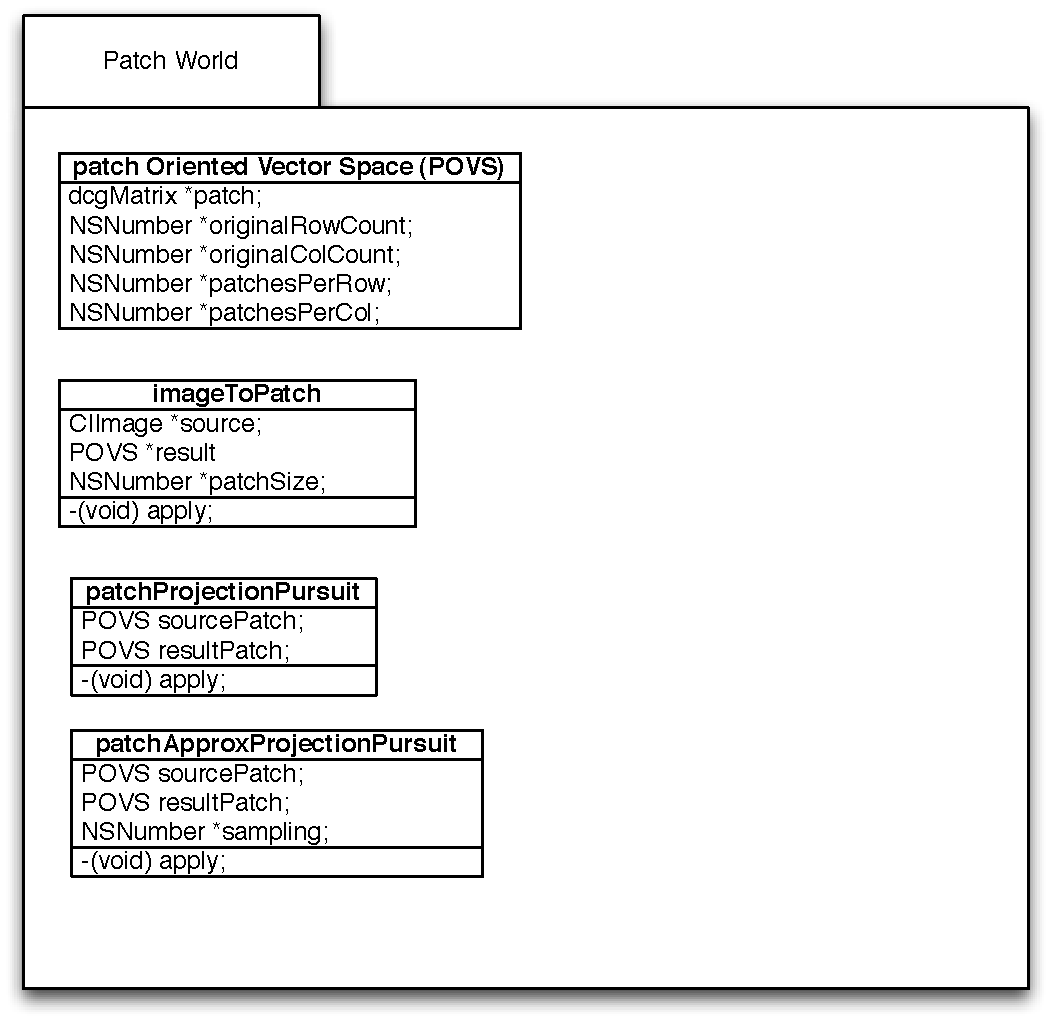
\includegraphics[width=4in]{patchWorld.pdf} 
%   \caption{Patch World Framework}
%   \label{fig-patch-world}
%\end{figure}


\subsubsection{Connection between Independent Component Analysis and Sparse Code Shrinkage}
\label{ica-scs-connection}

The constraints on Sparse Code Shrinkage are included in the following list.  Accompanying these requirements are comments that show the connection of Sparse Code Shrinkage to ICA. 
\begin{enumerate}
\item First, using a noise-free training set of $\vec{x}$, use some sparse coding method for determining the orthogonal matrix $\mathbf{W}$ so that the components $s_i$ in $\vec{s} = \mathbf{W}\vec{x}$ and so that $\vec{s}$ has as sparse a distribution as possible.  Estimate a density model $p_i (s_i)$ for each sparse component. 
\begin{itemize}
	\item Note that if $\vec{x}$ is already whitened, then the ICA mixing matrix is a transformation matrix satisfying the constraints on $\mathbf{W}$.
	\item The exponential and Laplace density functions are specific components to the non-polynomial projection pursuit family. 
\end{itemize}


\item Invert the relation $\vec{s} = \mathbf{W}\vec{x}$  to obtain estimates of the noise-free $\mathbf{x}$, given by $\mathbf{\hat{x}}(t) = \mathbf{W}^T \hat{\mathbf{s}}(t)$.
\end{enumerate}
The matrices $\mathbf{W}$ and $\mathbf{A}$ are mixing matrices.  Under the constraint that both  $\vec{s}$ and $\vec{x}$ are zero mean and unit variant, then $\mathbf{W}= \mathbf{A}^{-1} = \mathbf{A}^T$.



\bibliography{../patternNotes.bib}
\bibliographystyle{abbrv}
\end{document}